\chapter{Diskretisierung}

Partielle Differentialgleichungen (PDGn) n-ter Ordnung für skalares $u(x)$ sind von der Form
\begin{equation}
  F(x, t, u(x), Du(x), \dots, D^nu(x))=0, \qquad x\in\Omega\subset\mathbb{R}^d \; .
\end{equation}
Sie unterliegen Randbedingungen (für die Zeitvariable auch Anfangsbedingung genannt), die je nach Problemstellung auf Teilen des Randes formuliert sind. Beispielsweise ist die Auslenkung einer eingespannten Membran am Ortsrand fest, während in der Zeit lediglich für $t_0$ ein Randwert vorliegt (am linksseitigen Rand der Zeitdomäne).

Die LvNG \eqref{eq:lvn} ist eine lineare PDG zweiter Ordnung in $d=2$ Dimensionen. Sie ist weder elliptisch, noch parabloisch, noch hyperbolisch\footnote{Dies ist ersichtlich anhand der Eigenwerte der Koeffizientenmatrix zweiter Ableitungen $T=\text{diag}(0,1,-1)$ für Gleichung \eqref{eq:lvn_first}}.
Ferner bildet $u\in C^2(\Omega)$ in den Raum der komplexen Zahlen ab. Damit unterscheidet sich das Problem bereits grundlegend von den zumeist in der Literatur vorkommenden Problemstellungen. Die stationäre LvNG hingegen ist hyperbolisch. In diesem Kapitel soll ein Verfahren entwickelt werden, welches bislang noch nicht zur Anwendung gekommen ist im Kontext der LvNG: das \emph{Discontinuous-Galerkin}\index{Discontinuous-Galerkin Verfahren} (DG) Verfahren. Die Ausführungen orientieren sich an dem praxisnahen Buch von Hesthaven und Warburton \cite{buch}.

Zunächst wird ein Überblick über verschiedene, gängige numerische Verfahren gegeben. Vor- und Nachteile werden skizziert, wenngleich die Numerik partieller Differentialgleichungen ein großes Forschungsgebiet ist und somit die verschiedenen angedeuteten Probleme sich möglicherweise nur in einer oberflächlichen Betrachtung als solche äußern.

\section{Übersicht}\label{sec:Übersicht}
Bei der Diskretisierung einer PDG sind zwei grundlegende Fragestellungen zu berücksichten:
\begin{enumerate}
  \item Auf welche Weise wird die Lösung $u(x,t)$ durch eine diskrete Lösung $u_h(x,t)$ genähert?
  \item Wie ist die Verbindung zwischen diskretisierter Lösung und zugrundeliegender PDG?
\end{enumerate}
Als Folge einer unterschiedliche Beantwortung dieser Fragen wurden zahlreiche Verfahren entwickelt, die jeweils spezifische Vor- und Nachteile aufweisen. Im Folgenden werden in knapper Form drei Verfahren vorgestellt und  gegeneinander verglichen. In dieser Reihenfolge nimmt die Komplexität zu, denn die Schwächen des einen Verfahrens führen jeweils zu der nächst allgemeineren Formulierung.

\subsection{Finite Differenzen}\index{Finite Differenzen}\label{sec:FD}
Die partiellen Ableitungen werden bei diesem Verfahren durch eine endliche (finite) Anzahl von Differenzen genähert. Zur Formulierung der n-ten Ableitung einer Funktion $f(x)$ im Punkt $x_0$ wird die zugehörige Taylorreihe bis zur n-ten Ordnung verwendet. Der Punkt $x_0$ entstammt einem Gitter, welches das Gebiet $\Omega$ diskretisiert. Dieser Ansatz setzt inhärent voraus, dass eine Funktion sich hinreichend genau durch ein lokales Polynom niedriger Ordnung nähern lässt. Damit ist zeitgleich Frage (1) beantwortet.

Die Antwort auf die zweite Frage bestimmt dann die Koeffizienten der lokalen Polynome. Durch Einsetzen der Näherung $u_h(x,t)$ in die PDG folgt ein Residuum
\begin{equation}
  \mathcal{R}(x,t)\equiv F(x,t, u_h(x), Du_h(x), \dots, D^nu_h(x,t)) \; ,
\end{equation}
welches i.A. nicht verschwindet, denn sonst wäre ${u_h(x,t) = u(x,t)}$ die exakte Lösung. Zur Bestimmung der Koeffizienten (Freiheitsgrade) wird daher beispielsweise gefordert, dass auf den Gitterpunkten ${\mathcal{R}(x^k,t)=0}$ verschwindet.

Das Verfahren ist besonders leicht zu implementieren. Es ist robust, effizient und wird von einer umfangreichen Literatur gestützt. Für zeitabhängige Probleme folgt aus der Ortsdiskretisierung eine explizite semidiskrete Form, was eine Flexibilität in der Wahl der Zeitschritt-Methode ermöglicht. In höherdimensionalen Problemen $d>1$ erfordert das Verfahren jedoch eine Tensorprodukt-Struktur der Basisfunktionen, sodass letztlich komplexe Geometrien $\Omega\subset{\mathbb{R}^d}$ nicht gut abgebildet werden können. Ferner führen Unstetigkeiten in den Randbedingungen oder internen Schichten (wie zum Beispiel der Potentialsprung in Abbildung \ref{fig:pot1}) zu Problemen aufgrund der simplen, zugrundeliegenden Diskretisierung.

\subsection{Finite Volumen}\index{Finite Volumen}
Für erhöhte geometrische Flexibilität und insbesondere für nichtlineare Erhaltungsgleichungen eignet sich das Finitive Volumen (FV) Verfahren. Das Gebiet $\Omega$ wird dabei in Zellen aufgteilt, zumeist Simplizes. Die approximative Lösung $u_h(x,t)$ wird als Konstante $\bar{u}^k(t)$ innerhalb einer Zelle $k$ gesetzt. Die PDG wird lokal über jede Zelle integriert, wobei auftretende Divergenzterme mit Hilfe des Gaußschen Satzes in Oberflächenterme überführt werden. Für diese Terme müssen geeignete Flüsse gefunden werden und diese Wahl führt zu unterschiedlichen Verfahren. Da der Fluss in eine Zelle hinein demjenigen aus der Nachbarzelle heraus entspricht, sind die FV Verfahren konservativ.

Während wegen der Flexibilität bezüglich Geometrie und Wahl des Flusses die FV Verfahren sehr erfolgreich sind, offenbart die Forderung nach Verbesserung der Genauigkeit ein fundamentales Problem: im mehrdimensionalen müsste die geometrische Flexibilität wieder fallengelassen werden. Um nämlich $u_h(x,t)$ als Polynom vom Grad $N$ zu entwickeln und somit ${N+1}$ Koeffizienten zu finden, müssen zellübergreifende Informationen gesammelt werden aus mindestens ${N+1}$ Zellen (der sogenannten \emph{stencil} wird ausgeweitet). Dadurch wird eine spezielle Gitterstruktur erforderlich, weshalb geometrische Flexibilität nicht länger gewährleistet ist.

Im eindimensionalen Fall $d=1$ ist eine Erhöhung der Genauigkeit jedoch möglich und es soll an dieser Stelle betont werden, dass die LvNG ebenso mit einem zweistufigen FV Verfahren und Polynomgraden ${N_x,N_y > 1}$ gelöst werden kann. Die Flexibilität des Gitters ist im Falle eines hybdriden FV/DG-Verfahrens ohnehin nicht gegeben (vgl. Kapitel \todo{Referenz}).

\subsection{Finite Elemente}\index{Finite Elemente}
Der Übergang zu den Finite Elemente Methoden (FEM) geschieht, indem die approximative Lösung innerhalb einer Zelle nicht mehr als konstant gesetzt wird. Erhöhung der Genauigkeit durch Erhöhung der Freiheitsgrade ist dann ohne weiteres möglich, indem ähnlich wie beim FD Verfahren das Residuum auf den inneren Interpolationspunkten einer jeden Zelle orthogonal zu allen Testfunktionen sein soll (vgl. Kapitel \ref{sec:FEM}). Die numerische Lösung $u_h(x,t)$ wird also als lokales Polynom auf jeder Zelle angesetzt, wobei sogar der Polynomgrad von Zelle zu Zelle verschieden sein kann (sogenannte \emph{hp-adaptivity}). Die Wahl der Räume für Basis- und Testfunktionen führt zu unterschiedlichen FEM Verfahren. Werden an die Polynome zellübergreifende Stetigkeitsanforderungen gestellt, so führt dies zu den \emph{Continuous Galerkin} (CG)\index{Continuous Galerkin (CG)} Methoden.

Ein Nachteil ist hier für zeitabhängige Probleme die implizite Form der Massenmatrix, die eine Invertierung in jedem Zeitschritt erfordert. Ferner führen Schocks und Unstetigkeiten, wie sie in hyperbolischen Erhaltungsgleichungen auftreten können, zu Problemen \cite{dolejvsi2015discontinuous}. In FD- bzw. FV-Verfahren werden solche Umstände durch ein \emph{Upwind Scheme}\index{Upwind Scheme} bzw. einen \emph{Upwind Flux}\index{Upwind Flux} berücksichtigt. Indem die oben genannte Stetigkeitsanforderung fallen gelassen wird, lassen sich die Vorteile von FV und CG-FEM kombinieren durch die sogenannten  \emph{Discontinuous Galerkin}\emph{Discontinuous Galerkin (DG)} (DG) Methoden. Genau wie bei den FV Verfahren ist auch für die DG Methoden die Wahl eines geeigneten Flusses das Herzstück.

Die Abbildung \ref{fig:vergleich_hest} zeigt schematisch die Vor- und Nachteile der genannten Verfahren. Zahlreiche Entwicklungen und Erweiterungen überwinden die Nachteile häufig und es gibt daneben eine Reihe weiterer Eigenschaften, die zumeist problemabhängig sind und daher in dieser Übersicht nicht erwähnt werden können.
\todo{Scan}

\section{Einführung in die DG Methoden}
Die DG Methoden entstammen als erweiterte FE Methoden den abstrakten Varitationsproblemen. Motiviert wird ein solches Problem physikalisch durch die Minimierung einer Energie (mathematisch auch als Kostenfunktion bekannt). Für eine eingespannte Membran führt die Variationsrechnung beispielsweise zu den bekannten Euler-Lagrange Gleichungen. Das abstrakte Problem lautet stets:
\begin{equation}\label{varprob}
      \emph{Finde ein } u\in X\emph{ , sodass für alle } v\in X \emph{ gilt } a(u,v) = \ell(v).
\end{equation}
Hier ist $X$ ein Banach-Raum, $a:X\times X \rightarrow \mathbb{R}$ eine Bilinearform und ${\ell:X\rightarrow \mathbb{R}}$ ein lineares Funktional.
Der mit Abstand wichtigste Satz in diesem abstrakten Setting ist der Satz von Lax-Milgram \cite{buchPietro} über die Existenz und Eindeutigkeit einer Lösung (\emph{well posedness}). Dazu werden die Begriffe Koerzivität und Stetigkeit benötigt.
\begin{definition}[Koerzivität und Beschränktheit einer Bilinearform] \label{def:koerz}
  Sei $X$ ein Hilbertraum, $a \in \mathcal{L}(X\times X, \mathbb{R})$ und $b \in \mathcal{L}(X\times X, \mathbb{C})$. $a$ heißt koerzitiv auf $X$ falls es ein $\beta>0$ gibt sodass
  \begin{equation}
    \forall \, v \in X : \qquad \beta\norm{v}^2_X \leq a(v,v)
  \end{equation}
  $b$ heißt koerzitiv auf $X$ falls es ein $\beta>0$ gibt sodass
  \begin{equation}
    \forall \, v \in X : \qquad \beta\norm{v}^2_X \leq  \operatorname{Re}(b(v,v))
  \end{equation}
  a und äquivalent b heißen beschränkt falls es eine Konstante $C>0$ gibt sodass
  \begin{equation}
    \forall \, v,w \in X : \qquad C\norm{v}_X \norm{w}_X \geq |a(v,w)|
  \end{equation}
\end{definition}
\begin{satz}[Lax-Milgram]\label{laxmilgram}
  Sei $X$ ein Hilbertraum, $a \in \mathcal{L}(X\times X, \mathbb{R})$ und darüber hinaus ${\ell\in\mathcal{L}(X,\mathbb{R})=X^*}$. Dann ist das Variationsproblem \ref{varprob} well posed wenn die Bilinearform beschränkt und koerzitiv ist. Es gilt ferner die a priori Abschätzung
  \begin{equation}
    \norm{u}_X \leq \frac{1}{\beta} \norm{\ell}_{X^*}
  \end{equation}
\end{satz}
 Für eine PDG ergibt sich die variationale Formulierung (auch als \emph{schwache Formulierung}\index{schwache Formulierung} bezeichnet) mit ${X=W^{k,p}(\Omega)}$ aus einer Multiplikation mit einer Testfunktion ${w\in X}$ und Integration über die offene bschränkte Menge ${\Omega \subset \mathbb{R}^d}$ mit Lipschitz-Rand $\Gamma = \partial\Omega$.
 Dabei ist ${W^{k,p}(\Omega)}$ der Sobolev-Raum
 \begin{equation*}
   W^{k,p}(\Omega) \equiv \{ \varphi \in L^p(\Omega) \, : \, D^{\alpha}\varphi \in L^p(\Omega) \, \forall \, |\alpha| \leq k\}
 \end{equation*}
 mit Norm
 \begin{equation*}
   \norm{\Psi}_p = \left\{ \sum_{|\alpha|=k}\norm{D^{\alpha}\varphi}_p^p\right\}^{\nicefrac{1}{p}} \; .
 \end{equation*}
 Die \emph{schwache Lösung}\index{schwache Lösung} ist dann die Lösung dieser schwachen Form. Das Wort \emph{schwach} bezieht sich hierbei auf die schwächere Regularitätsanforderung, denn die Variationsformulierung kontrolliert die Ableitung nur in integraler Form, wie auch die Definition des Sobolev-Raums zeigt.

 Im Falle der LvNG wird zunächst abstrakt der Rand in Dirichlet-Rand $\Gamma_D$ mit ${u(x,t)|_{\Gamma_D} = g(x)}$ und Rest ${\Gamma\textbackslash\Gamma_D}$ unterteilt. In zwei Dimensionen $d=2$ ergibt sich
 \begin{align}
              i \int_{\Omega} \partial_t u(x,t) v(x,t) + \int_{\Omega}\operatorname{div}(A\nabla u(x,t)) v(x,t) - \int_{\Omega}B(x,t) u(x,t) v(x,t) = 0 \\
  \Rightarrow i \int_{\Omega} \partial_t u v - \int_{\Omega}(A\nabla u)\cdot\nabla v - \int_{\Omega}B u v + \int_{\Gamma\textbackslash\Gamma_D} n \cdot A\nabla u v = - \int_{\Gamma_D} n \cdot A\nabla g v \; .
 \end{align}
 Prinzipiell wird also alles, was nicht von der Lösung $u$ selbst abhängt, auf die rechte Seite geschrieben und als lineares Funktional $\ell(v)$ definiert.

 Die FE Methoden verarbeiten das analytische Varitationsproblem durch eine geeignete Diskretisierung. Folgende Schritte werden dabei vorgenommen:
\begin{enumerate}[label=(\roman*)]
  \item Die abstrakten Sobolev-Räume werden durch endlich dimensionale Räume $X\fin$ approximiert.
  \item Es werden Basisfunktionen für den Raum $X\fin$ definiert.
  \item Das Gebiet $\Omega$ wird in Elemente $D^1,\dots, D^K$ einfacher Gestalt unterteilt. Hierdurch entsteht im zweidimensionalen die aus vielen Bildern bekannte Dreiecksstruktur komplizierter Oberflächen. Die Teilgebiete lassen sich durch einen Diffeomorphismus $F_k: \hat{K}\rightarrow D^k$ aus einem Referenzelement $\hat{K}$ erzeugen. So werden Integrale einmalig auf dem Referenzelement ausgewertet und dann über den Transformationssatz mit $F_k$ für das jeweilige Element ausgerechnet.
\end{enumerate}
Liegen nun Lösungs- und Testfunktionen in einem abgeschlossenen, nicht-leeren Teilraum $X\fin$ von $X$, so folgt erneut Existenz und Eindeutigkeit aus Beschränktheit und Koerzivität der Bilinearform auf $X$, wie sich leicht zeigen lässt. %(Thm 2.17)
Die diskrete Lösung $u\fin$ wird auch als \emph{Galerkin Näherung}\index{Galerkin Näherung} bezeichnet, denn die Prozedur geht auf Ritz, Galerkin und Bubnov im Jahre 1915 zurück. Eine Antwort auf die erste Frage des vorangegangenen Abschnittes nach dem Zusammenhang zwischen $u$ und $u\fin$ gibt das Lemma von Cea. Es trifft eine Abschätzung für $\norm{u\fin-u}_X$ und besagt außerdem, dass dieser Fehler umso besser ist, je besser $X\fin$ den Raum $X$ approximiert.

Die DG-Methoden zählen jedoch zu den \emph{nicht-konformen}\index{nicht-konforme Methode} Methoden, die sich dadurch unterscheiden dass $X\fin\not\subset X$. Dann lautet die diskrete Approximation des Variationsproblems
\begin{equation}
  \emph{Finde ein } u\fin\in X{\mathcal{T}}\emph{ , sodass für alle } v\fin\in X\fin \emph{ gilt } a\fin(u\fin, v\fin) = \ell\fin(v\fin)
  \label{approx_varprob}
\end{equation}
und es gilt das zweite Strang-Lemma als Analogon zum Lemma von Cea.
\begin{satz}[Zweites Strang-Lemma]\label{strang}
  Sei $u$ Lösung des Variationsproblems \ref{varprob}, und $u\fin$ die Ritz-Approximation mit koerzitivem $a \in \mathcal{L}(X\fin \times X\fin, \mathbb{C})$ und $\ell\fin \in \mathcal{L}(X\fin, \mathbb{C})$. Dann gilt
  \begin{equation}
    \begin{aligned}
    \norm{u-u\fin}_{X\fin} \leq &\left(1 +\frac{C\fin}{\beta\fin}\right) \inf_{v\fin \in X\fin}\norm{u-v\fin}_{X\fin} \\
    & +\frac{1}{\beta\fin} \sup_{w\fin \in X\fin: \norm{w\fin}=1} |a\fin(u,w\fin)-\ell\fin(w\fin)| \; .
  \end{aligned}
  \end{equation}
  Hierbei sind $\beta\fin$ und $C\fin$ Koerzivitäts- bzw. Stetigkeitskonstanten des approximierten Variationsproblems \ref{approx_varprob}.
\end{satz}
Die Existenz und Eindeutigkeit der Ritz-Approximation $u\fin$ ergibt sich wieder aus dem Satz von Lax-Milgram. Alternativ folgt aufgrund der endlichen Dimensionalität des Raumes $X\fin$ in Anbetracht der Linearität des Problems \ref{approx_varprob} die Existenz aus der Eindeutigkeit. Hierzu genügt es, die Koerzivität von $a\fin$ zu zeigen vgl. Kapitel \todo{Referenz Koerzivität}.

Für zeitabhängige Probleme wird in dieser Arbeit wie auch in den meisten Literaturquellen \cite{NLS} zunächst im folgenden Abschnitt \ref{sec:primal} das stationäre Problem als Variationsproblem formuliert und dessen \emph{well-posedness} gezeigt. Anschließend wird die Stabilität der Lösung untersucht, also das Vorzeichen der zeitlichen Änderung von $\norm{u\fin}$, siehe Abschnitt \ref{sec:stabilität}.

\todo{Residuum orthogonal zu Testfunktionen}


\section{DG-Verfahren für die LvNG}
Für zeitabhängige PDGn mit Dimensionalität $d>1$ gibt es prinzipiell zwei verschiedene Möglichkeiten der Diskretisierung.
\begin{itemize}
  \item Die jeweiligen Orts-Koordinaten werden sukzessive behandelt -- dieses Vorgehen wird als \emph{Methode der Geraden}\index{Methode der Geraden} bezeichnet. Dabei können die einzelnen Richtungen auch mit unterschiedlichen Methoden diskretisiert werden, was im Folgenden als \emph{Hybridverfahren}\index{Hybridverfahren} bezeichnet werden soll. Das resultierende Gitter ist stets ein Rechteckgitter, was wie bereits in Kapitel \ref{sec:FD} erwähnt geometrische Flexibilität nicht zulässt. Andererseits ist dies für rechteckige Gebiete $\Omega$ unkritisch.
  \item Die Orts-Koordinaten werden mit einem einzigen Verfahren diskretisiert -- die Basisfunktionen ergeben sich dann nicht mehr aus einem Tensorprodukt, sondern sind direkt $d$-dimensional.
\end{itemize}
Die Abbildung \ref{fig:methodeDerGeraden} veranschaulicht das Vorgehen.
\begin{figure}
  \centering
  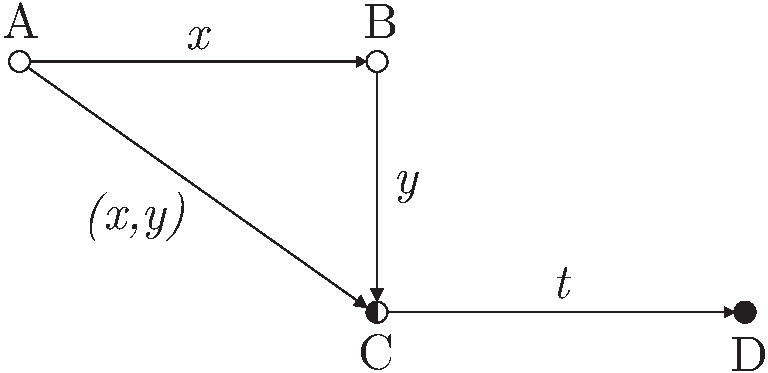
\includegraphics[width=0.7\textwidth]{files/methodeDerGeraden.pdf}
  \caption{Zwei verschiedene Möglichkeiten, zur semidiskreten Form C zu gelangen. Der Weg über B entspricht dabei der \emph{Methode der Geraden}. Im Punkt C verbleibt ein System gewöhnlicher DGLn, welches mit einem geeigneten Zeitschrittverfahren gelöst wird.}
  \label{fig:methodeDerGeraden}
\end{figure}
In Anbetracht der Randbedingungen aus Kapitel \ref{sec:RB} ist das Hybdriverfahren ein intuitiverer Zugang, denn die Randbedingungen können nicht einfach als Dirichlet-Randbedingungen auf $\Gamma$ gesetzt werden. Stattdessen ist eine Unterscheidung hinsichtlich der Geschwindigkeit notwendig, was wiederum eine Diagonalisierung des Ableitungsoperators $\partial_y$ erfordert. Diese Diagonalisierung lässt sich mit der Methode der Geraden separieren von der $x$-Diskretisierung, vergleiche auch die Ausführungen in \cite{lukas1}. Die Diagonalisierung entspricht letztlich einer Fourier-Transformation (FT), denn im Impulsraum ist der Ableitungsoperator  diagonal. Eine DG-Diskretisierung bzgl. $y$ hätte dabei jedoch zur Folge, dass die FT für \emph{double-valued}\footnote{An double-valued Punkten ist der Funktionswert nicht eindeutig definiert. Es gibt jeweils einen zu Element 1 und einen zu Element 2 zugehörigen Wert, siehe auch Abbildung \ref{fig:notation_DG}.} Punkte ausgewertet werden muss.

Eine weitere Motivation für das Hybdriverfahren ist die Charakteristik der PDG nach erfolgter $y$-Diskretisierung. Dann liegt nämlich ein System von Advektions-Reaktions-Gleichungen vor, was wiederum den Transportcharakter der PDG offenbart. DG-Verfahren sind wie bereits in Abschnitt \ref{sec:Übersicht} angesprochen dank einer flexiblen Wahl des numerischen Flusses für eben solche Transportgleichungen ausgelegt.

In einem vorbereitenden Einschub sollen im Folgenden einige wichtige Erkenntnisse aus der Theorie für Riemann Probleme hyperbolischer Systeme gezeigt werden. Sie werden später in Abschnitt \ref{sec:Hybridverfahren} benötigt, um einen korrekten numerischen Fluss zu formulieren.

\subsection{Riemann Probleme in hyperbolischen Systemen}\label{sec:riemann}\index{Riemann Problem}
Die folgenden Ausführungen orientieren sich an dem Buch von Leveque \cite{buchLeveque}.
Das Riemann Problem für die skalare Adventkionsgleichung $u_t + f_x(u) = 0$ mit dem Fluss $f(u(x)) = s u(x)$ ist durch die diskontinuierliche Anfangswertbedingung
\begin{equation}
  u(x,0) = \begin{cases} u^- , \; x < 0 \\
                         u^+ , \; x > 0
           \end{cases}
\end{equation}
gestellt.  Die \emph{Rankine-Hugoniot-Bedingung}\index{Rankine-Hugoniot-Bedingung} lautet im skalaren Fall
\begin{equation}
  s(u^- - u^+) = (f^- - f^+) \; .
  \label{eq:rhc}
\end{equation}
Die Größe s ist dabei die Geschwindigkeit, mit der sich die Diskontinuität ausbreitet (\emph{shock speed}). Im allgemeineren Fall eines linearen Systems mit $f(u) = A u$ wird angenommen, dass die Matrix $A$ reelle, disjunkte Eigenwerte $\lambda_1 < \lambda_2 < \dots < \lambda_m$ hat, das heißt $A$ ist diagonalisierbar gemäß
\begin{equation}
  A = R \Lambda R^{-1}
\end{equation}
mit $R=[r_1 \, r_2 \, \dots \, r_m]$ als Transformationsmatrix mit den zugehörigen Eigenvektoren. Die Eigenwertgleichung lautet
\begin{equation}
  Ar_p = \lambda_p r_p \qquad \forall \, p=1,\dots, m
  \label{eq:EWeq_A}
\end{equation}
Durch die Zerlegung von $u^-$ und $u^+$ in die Eigenwertbasis gemäß
\begin{equation*}
  u^- = \sum_{p=1}^m \alpha_p r_p \qquad u^+ = \sum_{p=1}^m \beta_p r_p,
\end{equation*}
folgt mit $v = R^{-1}u$ und wegen der Charakteristik der Advektionsgleichung
\begin{equation*}
  v_p(x,t) = \begin{cases} \alpha_p , \; x - \lambda_p t < 0 \\
                           \beta_p  , \; x - \lambda_p t > 0
             \end{cases}
\end{equation*}
Bezeichnet $J(x,t)$ den größtmöglichen Index $p$, für den $x-\lambda_p t > 0$ gilt, so ist
\begin{align}
  u(x,t) = \sum_{p=1}^{J(x,t)} \beta_p r_p + \sum_{p={J(x,t)}+1}^m \alpha_p r_p \; .
\end{align}
Dieser Zusammenhang wird in Abbildung \ref{fig:torte} gezeigt.
\todo{Tortendiagramm S-66}
Die Lösung ist konstant innerhalb der einzelnen Segmente. Entlang der $p$-ten Charakteristik springt die Lösung jedoch. Mit der zu \ref{def:jump} äquivalenten Definition des Sprungs ${\jump{u}\equiv u^- - u^+}$ lässt sich
\begin{equation}
  -\jump{u_p} = (\beta_p - \alpha_p) r_p \; ,
  \label{eq:TortenJump}
\end{equation}
schreiben, wie der Abbildung zu entnehmen ist. Hier ist wieder die Rankine-Hugoniot-Bedingung analog zu Gleichung \eqref{eq:rhc} ersichtlich, denn es ist mit $f(u) = A u$
\begin{equation}
  \begin{aligned}
    \jump{f}_p &= A\jump{u}_p \stackrel{\eqref{eq:TortenJump}}{=} -(\beta_p - \alpha_p) A r_p \stackrel{\eqref{eq:EWeq_A}}{=}  -(\beta_p - \alpha_p) \lambda_p r_p \\
    &= \lambda_p \jump{u}_p \; .
  \end{aligned}
\end{equation}
Um nun den numerischen Fluss $f^*$ eines DG- oder FV Verfahrens zu bestimmen, ist $u$ an dem Ort $x=0$ auszuwerten (was in diesen Verfahren den Elementkanten entspricht). Daher könnnen entweder von $u^-$ ausgehend die Sprünge nach rechts oder von $u^+$ ausgehend die Sprünge nach links aufaddiert  werden. Folglich gilt
\begin{align}
  \label{eq:rhc_1}
  u(x=0) &= u^- + \sum_{\lambda_p < 0} (\beta_p - \alpha_p)r_p = u^+ - \sum_{\lambda_p > 0} (\beta_p - \alpha_p)r_p \\
  \Rightarrow \qquad u(x=0) &= \frac{u^- + u^+}{2} + \frac{1}{2}\left( \sum_{\lambda_p < 0} (\beta_p - \alpha_p)r_p - \sum_{\lambda_p > 0} (\beta_p - \alpha_p)r_p \right) \; .
\end{align}
Multiplikation mit $A=R\Lambda R^{-1} = R(\Lambda^+ + \Lambda^-)R^{-1}$ (hierbei enthält $\Lambda^{+(-)}$ ausschließlich die positiven (negativen) Eigenwerte von $\Lambda$) ergibt den numerischen Fluss
\begin{align*}
  f^* = A \avg{u} + \frac{1}{2}& (R(\Lambda^+ + \Lambda^-)R^{-1}) \sum_{\lambda_p < 0} (\beta_p - \alpha_p)r_p \\
                     - \frac{1}{2}& (R(\Lambda^+ + \Lambda^-)R^{-1}) \sum_{\lambda_p > 0} (\beta_p - \alpha_p)r_p \\
         = A \avg{u} + \frac{1}{2}&\left( R\Lambda^-R^{-1} \sum_{\lambda_p < 0} (\beta_p - \alpha_p)r_p
                    - R\Lambda^+R^{-1} \sum_{\lambda_p > 0} (\beta_p - \alpha_p)r_p        \right) \; .
\end{align*}
Die letzte Gleichheit folgt aus $\sum_j (R^{-1})_{i,j} (r_p)_j = \delta_{i,p} e_p$ (mit $e_p$ als Einheitsvektor). Im Folgenden soll mit $|A|$ die Kurzschreibweise für $(|A|)_{i,j} = |A_{i,j}|$ verwendet werden. Dann lässt sich der Fluss weiter zusammenfassen:
\begin{align}
  f^* &= A \avg{u} + \frac{1}{2} \left( -R|\Lambda^-|R^{-1} \sum_{\lambda_p < 0} (\beta_p - \alpha_p)r_p
              - R\Lambda^+R^{-1} \sum_{\lambda_p > 0} (\beta_p - \alpha_p)r_p        \right) \\
        &= A \avg{u} - \frac{1}{2} \underbrace{(R|\Lambda^-|R^{-1} + R\Lambda^+R^{-1})}_{=R|\Lambda|R \equiv |A|}  \sum_p(\beta_p - \alpha_p)r_p   \\
        &\stackrel{\eqref{eq:rhc_1}}{=} A \avg{u} - \frac{1}{2} |A| (u^+-u^-) \\
        &= A \avg{u} + \frac{1}{2} |A| \jump{u}
\end{align}
Die gesamte Argumentation funktioniert auch, wenn A bereits diagonal ist. Am Ausgangspunkt der vektoriellen Advektionsgleichung wird direkt eine Transformation $u=Rv$ durchgeführt, sodass
\begin{align}
  v_t + \Lambda v_x = 0 \; .
\end{align}
Es folgt dann wie oben gezeigt der numerische Fluss
\begin{align}
  f^* = (\Lambda v)^* = \Lambda\avg{v} + \frac{1}{2}|\Lambda|\jump{v} \; .
  \label{eq:FLUX}
\end{align}


\subsection{DG/FV Hybridverfahren}\label{sec:Hybridverfahren}
In natürlichen Einheiten kann die bezüglich $y$ diskretisierte LvNG \eqref{eq:lvn} allgemein durch
\begin{equation}
  {A}^y u_t(x,t) + {B}^y u_x(x,t) + {C}^y(x,t)u(x,t) = 0
  \label{eq:qschema}
\end{equation}
geschrieben werden. Die Matrizen  ${A}^y$, ${B}^y$ und ${C}^y$ resultieren in diesem Abschnitt aus einem FV Verfahren, können aber ebenso anderen Verfahren entstammen.

Dem FV Ansatz in \cite{lukas1} folgend wird das Intervall ${[-L_y/2,+L_y/2]}$ in $K_y$ Zellen unterteilt. Hieraus ergeben sich demnach $K_y+1$ \emph{interfaces}
\begin{equation*}
  {y_{\nicefrac{1}{2}}, y_{\nicefrac{3}{2}}, \dots, y_{K_y + \nicefrac{1}{2}} = -L_y/2, -L_y/2+\Delta y_1,\dots,+L_y/2} \; .
\end{equation*}
Hierbei ist $\Delta y_i$ das Volumen der i-ten Zelle. Der Ansatz führt zu simplen Matrizen der Dimension ${K_y\times K_y}$ mit nicht verschwindenden Einträgen gemäß
\begin{equation}
  \begin{aligned}
  {A}^y_{i,i} &= \Delta y_i \\
  {B}^y_{i,i+1} &= -\frac{i}{2} \qquad
  {B}^y_{i+1, i} = +\frac{i}{2}  \\
  {C}^y_{i,i}(x,t) &= \mathrm{i} \frac{\Delta y_i}{4} (B(x, y_{i+\nicefrac{1}{2}},t) + B(x, y_{i-\nicefrac{1}{2}},t))  \\
  {C}^y_{i,i+1}(x,t) &= C^y_{i+1,i}(x,t) = \mathrm{i} \frac{\Delta y_i}{4} B(x, y_{i+\nicefrac{1}{2}},t)  \; .
  \end{aligned}
\end{equation}
Dieses Schema impliziert, dass $u(x,t)$ an den \emph{interfaces} als Mittelwert von rechts- und linksseitiger Zelle angenommen wird. Des weiteren sind  homogene Dirichlet Randbedingungen angenommen, also ${u(x,y_{\nicefrac{1}{2}}, t) = u(x,y_{K_y+\nicefrac{1}{2}}, t) = 0}$.

Die Matrix $B^y$ kann analytisch diagonalisiert werden. Es ist ${B^y = R\Lambda^y R^{\dagger}}$ mit der Diagonalmatrix
\begin{equation}
  \Lambda^y_{m,n} = \cos\left(\frac{2\pi n}{K_y+1}\right)\delta_{m,n}   \qquad m,n = 1,\dots,K_y
\end{equation}
und zugehörigen Eigenvektoren
\begin{equation}
  R_{m,n} = i^m \sin\left(\frac{mn\pi}{K_y +1} \right)   \qquad m,n = 1,\dots,K_y
\end{equation}
mti der Unitarität $R^{-1} = R^{\dagger}$.

Der Einfachheit halber wird nun $\Delta y_i = h_y$ konstant gesetzt, sodass
\begin{equation}
  (A^y)^{-1}B^y = h_y^{-1}R\Lambda^y R^{-1}
\end{equation}
gilt. Mit der unitären Transformation
\begin{equation}
  v(x,t) \equiv R^{\dagger}u(x,t)
\end{equation}
sowie der Definition
\begin{equation}
  G(x,t) \equiv h_y^{-1} R^{\dagger}C^y(x,t)
\end{equation}
folgt die diagonalisierte PDG
\begin{equation}
  v_t(x,t) + \Lambda^y v_x(x,t) + G(x,t)v(x,t) = 0 \; .
  \label{eq:diagLVN}
\end{equation}
Dies ist ein System von $K_y$ gekoppelten Advektions-Reaktions-Gleichungen mit Anfangsbedingung
\begin{equation}
  v(x,0) = (v(y_1,x,0),\dots,v(y_{K_y},x,0))^T = {v}_0(x) = R^{-1}u_0(x)
\end{equation}
und Fluss ${{f}({v}(x,t))=\Lambda^y {v}(x,t)}$. Sei ${\Omega_x = (-L_x/2,L_x/2)}$ ein beschränktes, offenes Gebiet mit Lipschitz Rand $\partial\Omega_x$ in  $\mathbb{R}$. Es wird durch die Vereinigung von $K_x$ nicht überlappenden Elementen ${D^k = [x_\ell^k,x_r^k]}$ trianguliert und diese Triangulierung sei mit $\mathcal{T}$ bezeichnet. Gesucht wird eine diskrete Lösung $v\fin$, welche Element des Finite-Elemente-Raumes
\begin{equation}
  V\fin = (V_{\mathcal{T},1})^{K_y} \equiv \left( \{ v \in L^1(\Omega_x) \;|\; v_h\rvert_{D^k} \in P_N(D^k) \, \forall \, k=1,\dots,K_x \} \right)^{K_y} \; ,
  \label{eq:FES}
\end{equation}
wobei $P_N$ der ${N+1=N_p}$ -dimensionale Raum der Polynome vom Grad $N$ ist. $V_{\mathcal{T},1}$ ist Teilmenge des gebrochenen Sobolev-Raumes
\begin{equation}
    H^1(\mathcal{T}) = \{ v \in L^2(\Omega_x) \, : \, v|_{D^k} \in H^1(D^k) \, \forall \, D^k \in \mathcal{T} \} \; ,
\end{equation}
welcher wiederum \underline{nicht} Teilmenge des Lösungsrames $X=H^1(\Omega)$ ist. Dies zeigt die Nicht-Konformität der Methode. Dennoch ist auch $H^1(\mathcal{T})$ Hilbertraum und es lässt sich der Satz von Lax-Milgram anwenden.

Der finite Elemente Raum \eqref{eq:FES} lässt Unstetigkeiten zu und diese werden gemäß Abbildung \ref{fig:notation_DG} gekennzeichnet. Werte am linken Rand eines Elementes bekommen den Index "+" und Werte am rechten Rand den Index "-".
\begin{definition}[Sprung und Mittelwert]\label{def:jump}
Es bezeichne $F=\cup_{D^k\in\mathcal{T}} \, \partial D^k$ die Menge aller Elementkanten. Auf inneren Kanten $e\in F_i=F  \textbackslash \partial\Omega_x$ werden
\begin{equation}
  \jump{u\fin}_e = u\fin^-|_e - u\fin^+|_e \qquad \avg{u\fin}_e = \frac{1}{2} (u\fin^-|_e + u\fin^+|_e)
\end{equation}
als Sprung $\jump{u\fin}_e$ und Mittelwert $\avg{u\fin}_e$ von $u\fin \in V\fin$ definiert. Auf den zwei äußeren Kanten $e\in F_e = F \textbackslash F_i$ wird diese Definition durch
\begin{equation}
  \jump{u\fin}_e \equiv \begin{cases} -u_{\mathcal{T},l}^+ \equiv -u\fin(x_{\nicefrac{1}{2}}^+) \; \text{, links}\\ u_{\mathcal{T},r}^- \equiv u\fin(x_{K_x+\nicefrac{1}{2}}^+) \; \text{, rechts} \end{cases}
   \qquad \avg{u\fin}_e = \begin{cases} u_{\mathcal{T},l}^+ \; \text{, links}\\ u_{\mathcal{T},r}^- \; \text{, rechts}\\  \end{cases}
\end{equation}
erweitert. Ganz analog werden Sprung und Mittelwert für $u \in V_{\mathcal{T},1}$ definiert. Damit gilt für alle Kanten $e\in F$ und $u,v\in V\fin$ die Relation
\begin{equation}
  \jump{u^{\dagger}v} = \jump{u}^{\dagger}\avg{v} + \avg{u}^{\dagger}\jump{v}
  \label{eq:jump_relation}
\end{equation}
\end{definition}
Um nun das DG Schema zu entwickeln, wird die Gleichung \eqref{eq:diagLVN} in die variationale Formulierung \eqref{eq:approx_varprob} gebracht. Gesucht sind Bilinearform a und Linearform $\ell$, an die folgende Anforderungen gestellt werden:
\begin{itemize}
  \item \emph{Konsistenz}\index{Konsistenz}: Für die schwache Lösung der LvNG und jede Funktion $v\in L^2(\Omega)$, die elementweise in $H^1(D^k)$ ist, gilt ${a\fin(u,v)=\ell\fin(v)}$.
  \item Beschränktheit und Koerzivität der Bilinearform nach Definition \ref{def:koerz}.
\end{itemize}
Der zweite Punkt ist diffizil und kann einzig durch eine gute Wahl des numerischen Flusses sichergestellt werden.
Konsistenz hingegen wird erreicht, indem zu der analytischen Form \eqref{eq:diagLVN} lediglich Sprungterme hinzugefügt werden, welche für die schwache Lösung $u\in H^1(\Omega)$ verschwinden. Der Grund hierfür liegt im zweiten Sobolevschen Einbettungssatz \cite{buchPietro}. Demnach bettet $W^{m,p}(\Omega)$ stetig in $C^{l,\alpha}(\overline{\Omega})$ ein, falls die Sobolev-Zahl ${\text{sob}(W^{m,p})\geq l+\alpha}$.
Insbesondere ist für $\Omega\in\mathbb{R}^1$ die Sobolevzahl $\text{sob}(H^1) = 1-\nicefrac{1}{2}$, weshalb $H^1$ stetig in $C^0$ einbettet. Für die schwache Lösung verschwinden also Sprungterme.

Multiplikation der diagonalisierten LvNG \eqref{eq_diagLVN} mit einer Testfunktion $\varphi\in V\fin$, Integration über ein Element $D^k$ und anschließende partielle Integration liefert
\begin{equation*}
  \int_{D^k} (\varphi^{\dagger} \partial_t v - \partial_x \varphi^{\dagger} f(v) + \varphi^{\dagger} G v) + \int_{\partial D^k}\hat{n}\varphi^{\dagger}f = 0 \; .
\end{equation*}
mit dem nach außen zeigenden Normalenvektor $\hat{n}$. Durch Summation über alle $K_x$ Elemente folgt
\begin{equation*}
  \sum_{D^k\in\mathcal{T}}\int_{D^k} (\varphi^{\dagger} \partial_t v - \partial_x \varphi^{\dagger} f(v) + \varphi^{\dagger} G v)
  + \sum_{e\in F_i}\int_{e}\jump{\hat{n}\varphi^{\dagger}f} + \sum_{e\in F_e}\int_e \jump{\varphi^{\dagger}f}  = 0 \; .
\end{equation*}
Nun wird Relation \eqref{eq:jump_relation} und die Stetigkeit der schwachen Lösung $v$ genutzt (${\jump{v}=\jump{f}=0}$).
\begin{equation*}
  \sum_{D^k\in\mathcal{T}}\int_{D^k} (\varphi^{\dagger} \partial_t v - \partial_x \varphi^{\dagger} f(v) + \varphi^{\dagger} G v)
  + \sum_{e\in F_i}\int_{e}\jump{\hat{n}\varphi^{\dagger}} f + \sum_{e\in F_e}\int_e \jump{\varphi^{\dagger}} f  = 0
\end{equation*}
An dieser Stelle wird die schwache Lösung $v$ durch ihre diskrete Ritz-Approximation $v\fin$ ersetzt. Das führt dazu, dass der Fluss $f\fin = f(v\fin)$ nicht mehr eindeutig definiert ist auf den Elementkanten. Er wird durch den \emph{single-valued} \emph{numerischen Fluss}\index{numerischer Fluss} $\hat{f}$ ersetzt. Dieser ergibt sich in sinnvoller Weise aus der Lösung des Riemann-Problems aus Abschnitt \ref{sec:riemann}, denn die Situation im DG-Verfahren entspricht gerade einem solchen Problem. Aufgabe des numerischen Flusses ist es, die Randbedingungen in einer schwachen Weise zu erzwingen. So sollte beispielsweise für positive Geschwindigkeiten $\lambda_j$ (als Eigenwerte von $\Lambda$) am linken Rand
\begin{equation*}
  (\hat{f}(g, v^+_l))_j = \lambda_j g(x=-L_x/2)
\end{equation*}
gelten und damit dem Upwind Charakter der PDG Rechnung getragen werden.
Zunächst ist der numerische Fluss einfach eine Funktion$ \hat{f}(u^-,u^+)$, welche den analytischen Fluss $f$ approximiert.





% Die in Abbildung \ref{fig:pot1} eingezeichneten Längen werden wie in \cite{lukas1} zu
% \begin{align}
%   L_1 &= \SI{6}{\nano\meter}\\
%   L_2 &= \SI{5}{\nano\meter}\\
%   L_U &= \SI{30}{\nano\meter} \; .
% \end{align}
% gewählt. Hierin ist $L_U$ die Länge, über der die Spannung $U$ abfällt.

% \todo{Idee: TF-Lösung für Überlagerung von l und r zeigen.}

% \section{Mathematische Aspekte der \lvn}
% Die eindimensionale Wellenfunktion $\Psi(x)$ eines Teilchens ist ein Vektor des unendlich-dimensionalen Hilbertraums $L^2(\mathbb{R})$ mit dem üblichen Skalarprodukt
% \begin{align}
%   \bra{\Psi}\ket{\Phi} = \int_{\mathbb{R}} \Psi^*(x)\Phi(x) \diff x \; .
% \end{align}
% Beschränken wir uns auf ein Rechengebiet $L$, so ist entsprechend $\Psi(x) \,\in\,L^2(L)$. Diskretisieren wir ferner das System, so wird der Hilbertraum endlichdimensional mit Dimension $N$. Dann ist die Dichtematrix in Gleichung \eqref{eq:lvn} eine Matrix der Form $\mathbb{C}^N \times \mathbb{C}^N$ und der Liouville-Operator ein "Superoperator" \cite{frensley2} der Form $(\mathbb{C}^N \times \mathbb{C}^N)\times(\mathbb{C}^N \times \mathbb{C}^N)$.
% Letztlich wird numerisch gesehen $N^2$ der Anzahl Freiheitsgrade entsprechen und die \lvn wird wieder eine Matrix-Vektor-Gleichung sein. Dazu wird $u(x,y)$ nicht als Matrix, sondern als Vektor der Länge $N^2$ geschrieben.
% \todo{Eigenschaften von B(x,y) und A. Hermitizität von $\mathcal{L}$ (frensley).}
